% Template for Elsevier CRC journal article
% version 1.2 dated 09 May 2011
%------------------------------------------

%% The '3p' and 'times' class options of elsarticle are used for Elsevier CRC
%% The 'procedia' option causes ecrc to approximate to the Word template
\documentclass[5p,times,procedia]{elsarticle}
\flushbottom



%% The `ecrc' package must be called to make the CRC functionality available
\usepackage{ecrc}
\usepackage{amsmath}

% JO bibliography:
%\usepackage[sorting=none]{biblatex} %biblatex -nope!
%\addbibresource{Bibliography.bib}   %biblatex -nope!
%\usepackage{natbib}                 %natbib.  -nope!
%\bibliographystyle{unsrtnat}        %unsrtnat -nope!

% Jo color definition:
\usepackage{xcolor}
\definecolor{notecolor}{rgb}{0.16, 0.67, 0.53}

% JO note environment:
\newenvironment{note}{%
	\noindent
    \color{notecolor}%
}{%
    \par\medskip%
}

\usepackage{eurosym}




%% set the volume if you know. Otherwise `00'
\volume{00}

%% set the starting page if not 1
\firstpage{1}

%% Give the name of the journal
\journalname{Procedia CIRP}

%% Give the author list to appear in the running head
%% Example \runauth{C.V. Radhakrishnan et al.}
\runauth{Author name}

%% The choice of journal logo is determined by the \jid and \jnltitlelogo commands.
%% A user-supplied logo with the name <\jid>logo.pdf will be inserted if present.
%% e.g. if \jid{yspmi} the system will look for a file yspmilogo.pdf
%% Otherwise the content of \jnltitlelogo will be set between horizontal lines as a default logo

%% Give the abbreviation of the Journal.
\jid{trpro}

%% Give a short journal name for the dummy logo (if needed)
%\jnltitlelogo{Transportation Research}

%% Hereafter the template follows `elsarticle'.
%% For more details see the existing template files elsarticle-template-harv.tex and elsarticle-template-num.tex.

%% Elsevier CRC generally uses a numbered reference style
%% For this, the conventions of elsarticle-template-num.tex should be followed (included below)
%% If using BibTeX, use the style file elsarticle-num.bst

%% End of ecrc-specific commands
%%%%%%%%%%%%%%%%%%%%%%%%%%%%%%%%%%%%%%%%%%%%%%%%%%%%%%%%%%%%%%%%%%%%%%%%%%

%% The amssymb package provides various useful mathematical symbols
\usepackage{amssymb}


% if you have landscape tables
\usepackage[figuresright]{rotating}
%\usepackage{harvard}
% put your own definitions here:x
%   \newcommand{\cZ}{\cal{Z}}
%   \newtheorem{def}{Definition}[section]
%   ...

% add words to TeX's hyphenation exception list
%\hyphenation{author another created financial paper re-commend-ed Post-Script}

% declarations for front matter

\usepackage[bookmarks=false]{hyperref}
    \hypersetup{colorlinks,
      linkcolor=blue,
      citecolor=blue,
      urlcolor=blue}


\begin{document}
\begin{frontmatter}



%% Title, authors and addresses

%% use the tnoteref command within \title for footnotes;
%% use the tnotetext command for the associated footnote;
%% use the fnref command within \author or \address for footnotes;
%% use the fntext command for the associated footnote;
%% use the corref command within \author for corresponding author footnotes;
%% use the cortext command for the associated footnote;
%% use the ead command for the email address,
%% and the form \ead[url] for the home page:
%%
%% \title{Title\tnoteref{label1}}
%% \tnotetext[label1]{}
%% \author{Name\corref{cor1}\fnref{label2}}
%% \ead{email address}
%% \ead[url]{home page}
%% \fntext[label2]{}
%% \cortext[cor1]{}
%% \address{Address\fnref{label3}}
%% \fntext[label3]{}

\dochead{57th CIRP Conference on Manufacturing Systems 2024 (CMS 2024)}

\title{Digital Twin Based Online Material Defect Detection for CNC-Milled Workpieces}

%% use optional labels to link authors explicitly to addresses:
%% \author[label1,label2]{<author name>}
%% \address[label1]{<address>}
%% \address[label2]{<address>}



\author[a,b]{Johannes Kimmle} 
\author[a,c]{Dominik Lucke\corref{cor1}}%$\ast$}} %{cor1}
\author[b]{Konrad von Leipzig}
%\ead{author@institute.xxx}

\address[a]{ESB Business School, Reutlingen University, Alteburgstra\ss e 150, 72762 Reutlingen, Germany}
\address[b]{Department of Industrial Engineering, Stellenbosch University, Joubert Street, Stellenbosch, 7600, South Africa}
\address[c]{Fraunhofer Institute for Manufacturing Engineering and Automation IPA, Nobelstra\ss e 12, 70569 Stuttgart, Germany}

\aucores{* Corresponding author. Tel.: +49-7121-271-5005; fax: +49-7121-271-90-5005. E-mail address: dominik.lucke@reutlingen-university.de}

\begin{abstract}
Achieving reliable lot size one compatible and adaptable online quality monitoring for CNC-milled workpieces remains elusive yet.
To address this challenge, our approach aims to bridge the current gap in research by developing a cost-effective and reference-independent monitoring concept for material defect detection in CNC-machined parts. This paper presents a novel digital twin-based method, utilising machining vibrations and a g-code-based encoding of the cutting process. The objective is to detect material defects, such as blowholes, without the need for individual workpiece references. The proposed method aims to reduce barriers to entry, minimise waste, and enhance machine productivity by enabling automated early online quality control. To develop and validate the model, we generate a new dataset combining machining vibration with technological context data such as chip-shape. We demonstrate the feasibility and potential of the approach in a job shop setting on a 3-axis CNC mill.
\end{abstract}

\begin{keyword}
 Online process monitoring \sep Material defect detection \sep Digital Twin \sep Lot size one \sep Vibration monitoring

%old: Monitoring \sep Machining \sep Material defects \sep Vibrations \sep Lot size one

%% keywords here, in the form: keyword \sep keyword

%% PACS codes here, in the form: \PACS code \sep code

%% MSC codes here, in the form: \MSC code \sep code
%% or \MSC[2008] code \sep code (2000 is the default)

\end{keyword}
\cortext[cor1]{Corresponding author. Tel.: +49-7121-271-5005; fax: +49-7121-271-90-5005. E-mail address: dominik.lucke@reutlingen-university.de}

\end{frontmatter}


%=====================================================================
%=====================================================================
\section{Introduction}\label{Sec_Introduction}


The manufacturing industry is undergoing a paradigm shift, transitioning from a focus on 'responsiveness' to a 'market-of-one', deemed 'Mass Individualisation' \cite{Lu.Xu.ea2020} or 'Mass Personalisation' \cite{Qin.Lu2021}. This entails the production of custom-made products while maintaining the low unit costs traditionally associated with mass production.
In response, there has been a global push towards smart manufacturing characterized by autonomous operations enabled by advanced sensing, data processing, and decision-making technologies. \cite{Gu.Koren2022, Lu.Morris.ea2016}.

%While Additive Manufacturing (AM) can counter some of these challenges it is inferior to traditional Numerical Controlled machine tools (CNCs) such as milling machines concerning Dimensional accuracy, limited types of usable material, or low productivity. \cite{Chen.Lin2017,zotero-232,zotero-236} Hence, CNC processes will remain pivotal in manufacturing environments, offering great potential for optimisation due to their widespread adoption.  

Within this context, reducing lot sizes in job-shop settings becomes imperative, and additive manufacturing (AM), particularly 3D printing, emerges as a promising solution due to its autonomy and versatility.
However, despite its advantages, AM still falls short compared to traditional techniques like CNC milling in aspects such as dimensional accuracy, mechanical properties, material variety, and surface quality \cite{Chen.Lin2017,zotero-232,zotero-236}.
CNC milling, therefore, remains pivotal, presenting not only significant potential but also high necessity for optimisation due to its complex nature of underlying processes that result in lower process resilience and robustness compared to AM.

%\vspace*{8pt}
\begin{nomenclature}
\begin{deflist}[AAA]%number of letters
\defitem{CNC}\defterm{Computerised Numerical Controled (machine tool)}
\defitem{AM}\defterm{Additive Manufacturing}
\defitem{CCC}\defterm{...}
\end{deflist}
\end{nomenclature}%\vskip24pt

%idea:
%\begin{note}
%	- monitoring system to make make cnc machines more resilient and robust in a lot size one production scenario\\
%	- focussing on workpiece monitoring, specifically material defects and user error (at setup, like wrong part material, or part clamping error)
%\end{note}

%\subsection{Technical and economic demand}
A monitoring system that utilises deep process context (e.g. technological, geometric, or material property data) to generate reference agnostic (= lot size one capable) process status insights, would ready CNC mills for the Mass Personalisation paradigm shift.

Such a workpiece-centered monitoring system which detects material defects or user (=operator) error (e.g. wrong material, or part clamping error) during normal machining can increase process efficiency \& reliability, reduce waste, and enable higher product quality.  

To achieve economic efficiency and general market accessibility such a system must be easy to integrate, be machine agnostic, and be relatively low cost.

 
%=====================================================================
\section{Related work}
\begin{note}
	state of the art (1,5seiten)

\end{note}

%Machine tool and machine tool control munafacturers integrate all kind of monitoring capabilities in their products. Modern CNC mills are usually factory-fitted with spindle and axis drive energy meters where spindle tourque and axis resistance can be estimated from.

%Most of these focus on tool wear, surface finish optimisation, or machine maintenance. 
%Holistic process specific monitoring especially of the workpiece is rarely employed on today's shop floors or in current research.\\

%Almost exclusively CNC monitoring is focused on tool condition monitoring (especially tool wear and breakage), surface finish quality (including chatter), and machine health monitoring (within the scope of predictive maintenance) .
Predominantly, CNC monitoring is focused on tool condition monitoring, particularly detecting tool wear and breakage, ensuring surface finish quality, including mitigating chatter, and monitoring machine health for predictive maintenance purposes \cite[p.2727]{Kuntoglu.Salur.ea2021}.

The following sensors are used and listed with their general purpose below:
Table \ref{Tab_Sensors} lists employed sensors and rates them by investment cost and by information value.

\begin{table}[h]
\caption{Sensors according to signals and properties\cite[according to][p.2725]{Kuntoglu.Salur.ea2021}}
\label{Tab_Sensors}
\begin{tabular*}{\hsize}{@{\extracolsep{\fill}}lll@{}}
\toprule
Sensor & Level of investment cost & Extent of signal accuracy\\ && and information value\\
\colrule
Dynamometer    & $\bullet$\hspace{.5mm}$\bullet$\hspace{.5mm}$\bullet$\hspace{.5mm}$\bullet$\hspace{.5mm}$\bullet$\hspace{.5mm}   & $\bullet$\hspace{.5mm}$\bullet$\hspace{.5mm}$\bullet$\hspace{.5mm}$\bullet$\hspace{.5mm}$\bullet$\hspace{.5mm}\\
Accelerometer  &   $\bullet$\hspace{.5mm}$\bullet$\hspace{.5mm}$\bullet$\hspace{.5mm}$\bullet$\hspace{.5mm}   &  $\bullet$\hspace{.5mm}$\bullet$\hspace{.5mm}$\bullet$\hspace{.5mm}\\
AE             & $\bullet$\hspace{.5mm}$\bullet$\hspace{.5mm}$\bullet$\hspace{.5mm}$\bullet$\hspace{.5mm}     & $\bullet$\hspace{.5mm}$\bullet$\hspace{.5mm}$\bullet$\hspace{.5mm} \\
Current/power  & $\bullet$\hspace{.5mm}      & $\bullet$\hspace{.5mm}  \\
Temperature    & $\bullet$\hspace{.5mm}$\bullet$\hspace{.5mm}$\bullet$\hspace{.5mm}      & $\bullet$\hspace{.5mm}$\bullet$\hspace{.5mm}  \\
Sound          & $\bullet$\hspace{.5mm}      & $\bullet$\hspace{.5mm}  \\
\botrule 
\end{tabular*}
\end{table}


\vspace*{-\baselineskip}
\subsection{Related scientific work}
\vspace*{-\baselineskip}


\href{https://www.matta.ai/greymatta}{Matta's Grey-1 model} as shown in their paper \cite{Brion.Pattinson2022} demonstrates AM process monitoring on fused layer deposit 3D printers, based on an automated deep process understanding. 
They trained a multi head transformer model on labeled images, such as: extrusion speed, layer thickness and hotend temperature. They are able to detect extrusions errors (which translate in to material defects), or adjust printing parameters fully autonomously for unseen material.\cite{Brion.Pattinson2022}

This study serves as a substantial inspiration and influence for the present work.


Another notable study \cite{Pfirrmann.Baumann.ea2021} investigates the cutting forces measured by a (6-axis) dynamometer in micromanufactuirng of Ti6246 alloy by comparing them with theoretical calculted forces, to detect material defects such as blow holes.
This aproach is in theory lot size one capable because the force measurement is not compared to one of a part prior, but is rather based on experimental measurements and a geometric physically-based process simulation. It is concluded that the accuracy of the calculated force and the insufficient change of amplitude while machining a defect were to low to achieve automated detection. \cite[p.169]{Pfirrmann.Baumann.ea2021} 

While dynameter force measurements offer greatest signal accuracy and information value due to their direct measurement methode and process proximity \cite[]{Korkmaz.Yasar.ea2020}, they are the most expensive ($\sim 60.000$\euro) and usualy difficult to setup and not feasable for production envirnoments.



\begin{note}
Sensor products employed in research:

- Acoustic Emission via Optimizer 4D by Quass; powerful AE monitoring employed in tool condition monitoring and tested (sci) on chatter detection (Szulewski.Sniegulska-Gradzka2017)

- multi axis Force Dynanometers by Kistler; most direct process monitoring (most powerful); material defects monitoring in micro milling Ti(Pfirrmann.Baumann.ea2021)

- Contact Microphone (Gitarrenabnehmer) for chatter detection
\end{note}






%=====================================================================
\section{Aproach}
\begin{note}
	(vorgehen + prinzipielle aufbau/Konzept)\\
	- welche physikalische grösse? vibration\\
	- kontext architektur (feature)\\
	- schaubild design\\
	
\end{note}




%=====================================================================
\section{Implementation}

\begin{note}
- full design from approach transform to proof of concept\\
- in python, auf emco, DoE...\\
- experimental setup	
\end{note}

\begin{figure*}[t]
    \centering
    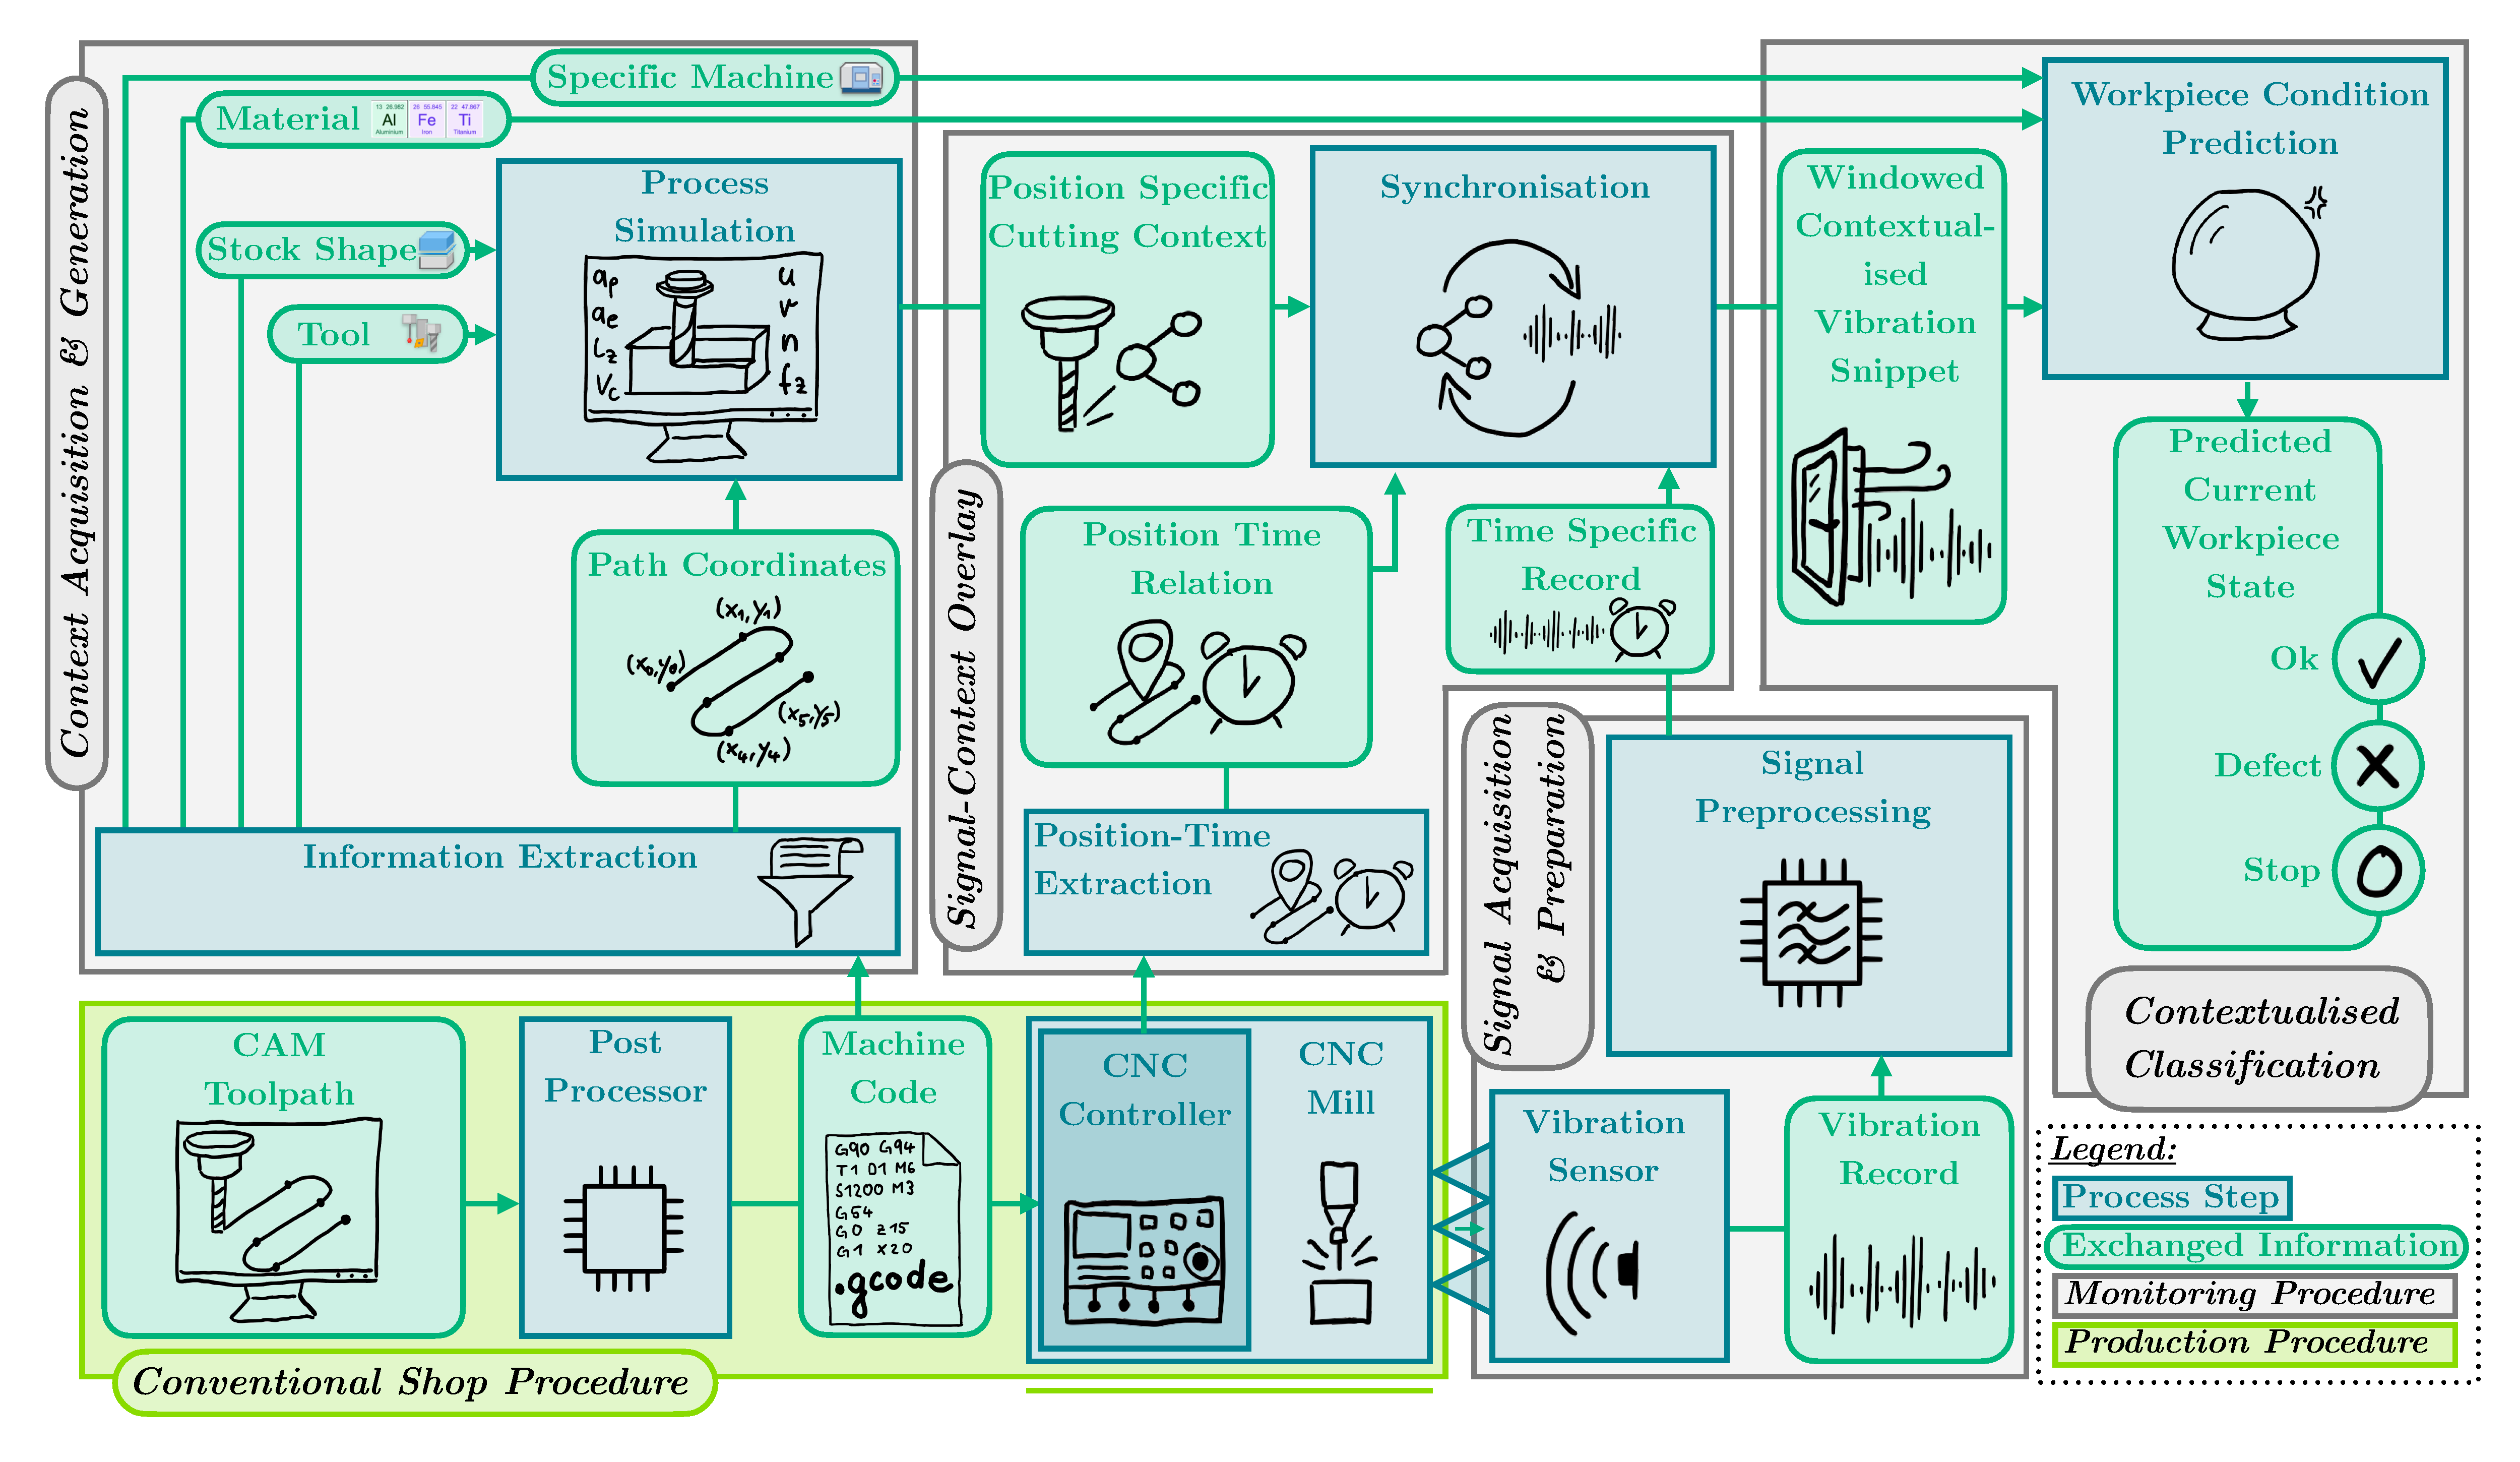
\includegraphics[width=0.99\linewidth]{ConceptDiagram.pdf}
    \caption{High-Level Concept}
    \label{Fig_ConceptDiagram}
\end{figure*}
 
 
%=====================================================================
\section{Validation}
\begin{note}
	...and evaluation

\end{note}
%=====================================================================
\section{Conclusion}
\begin{note}
	and futere recommendation (halbe seite)
	
\end{note}






Zitiertest...

\cite{Al-Naggar.Jamil.ea2021,Axinte.Gindy2004a,Ma.Howard.ea2020}

\cite{Axinte.Gindy2004a}

\cite{Ma.Howard.ea2020}

\cite{Biermann.Zabel.ea2013}

\cite{Chen.Lin2017}

%=====================================================================
%=====================================================================
%% For references without a BibTeX database:
% JO bibliography
%\printbibliography               %biblatex -nope!
\bibliographystyle{elsarticle-num} %elsevierspecific -yep!
\bibliography{Bibliography.bib} %natbib %elsevier is based on natbib -so yep!

\end{document}
